\section{Process Perspective}

\subsection{The Team's Setup}
Interaction between team members is a hybrid of physical meetings onsite at ITU and online meetings via Discord.  

During the project's preliminary phase, the team defined guidelines for a distributed workflow to be followed. The guidelines address how the team  utilizes Trunk Based Development \cite{trunkdev}, defines when a contribution is considered done, ascribes responsibility for integrating and reviewing these contributions, and how to document knowledge acquisition.

The workflow comprises of three phases; Planning, development, and release.
In the first two phases we prefer synchronous communication to simplify coordination.
The team discusses, defines, and distributes tasks for completing the week's working during the planning phase.
Thereafter, the tasks are managed on a GitHub project board (see \autoref{app:kanbamps}).
In the development phase tasks are delegated to one to two members.
When possible pair programming is used to be more productive \cite{strengthcasepairprog}.
Hence, the team has a clear overview of everyone's tasks and their progress during the development and release.
This reduces the need for communication as a method of coordination since the project board is a single source of work.

\subsection{CI/CD Chains}
\autoref{fig:quality_gates} below shows the series of quality gates that are part of the CI pipeline.

\begin{figure}[H]
    \centering
    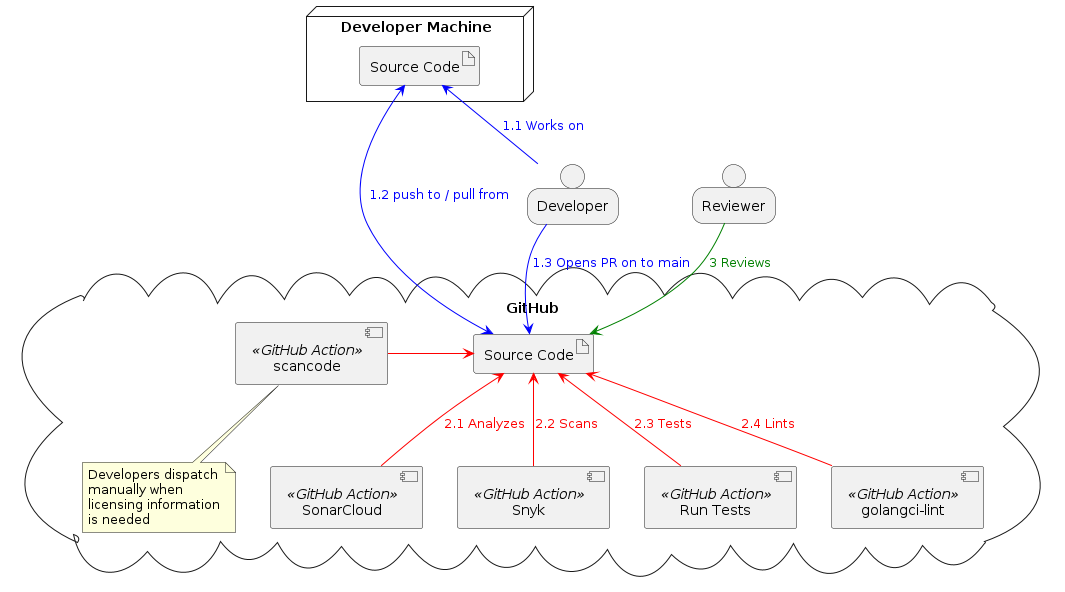
\includegraphics[scale=0.35]{images/cicd/quality_gates.png}
    \caption{A Diagram of \textit{Minitwit's} CI/CD pipeline}
    \label{fig:quality_gates}
\end{figure}

We employ quality gates to ensure high levels of code quality and security.
First, we use Git and GitHub for version control in a distributed work setting.
Once a developer is satisfied with their work, they open a pull request to merge the changes into main.
There are four quality gates that a PR must meet before it can be merged.
The pull request must then be reviewed and approved by another developer.
This bakes code reviews into our way of working.
Additionally, golangci-lint and SoncarCloud provide different perspectives on the quality of the code.
Furthermore, Snyk scans the repository for security vulnerabilities providing increased confidence that the code is safe for production.
Finally, the PR must also pass the test suite.
Although not automated, we have made it effortless to gain licensing information through the scancode GitHub action.

\autoref{fig:cicd} below shows the build and deployment steps that are part of our CI/CD pipeline.

\begin{figure}[H]
    \centering
    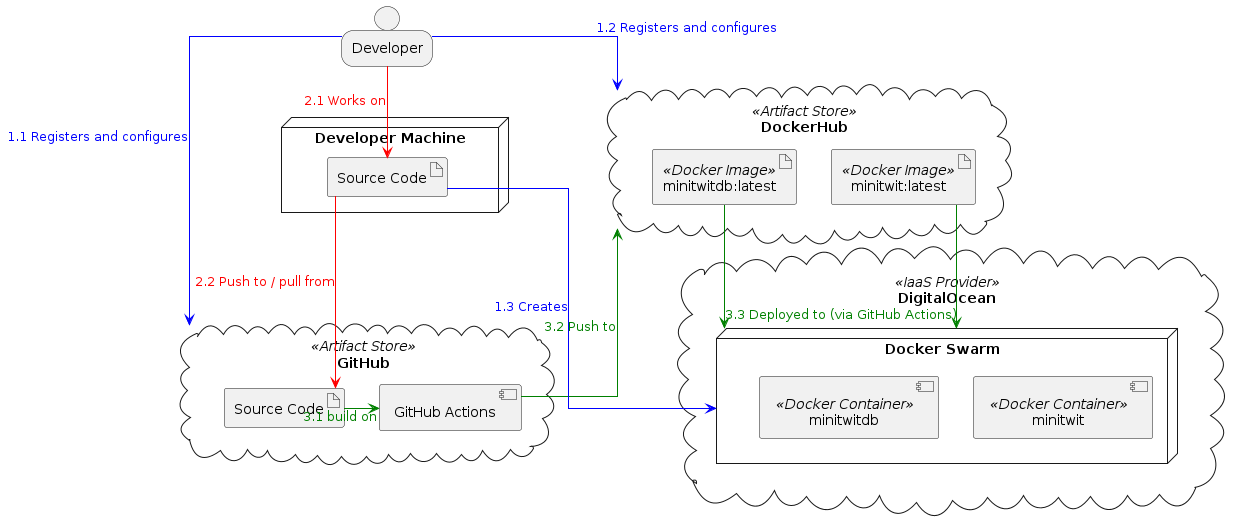
\includegraphics[scale=0.35]{images/cicd/cicd.png}
    \caption{A Diagram of \textit{Minitwit's} CI/CD pipeline}
    \label{fig:cicd}
\end{figure}

When a new feature is on the main branch, it will be included in the next weekly release.
When we make a release on GitHub, the main branch is built using GitHub actions and packaged into docker images. 
Dockerhub acts as an artifact store for these images.
Then GitHub actions will act on the Swarm Leader to pull the new images into the Docker Swarm using a rolling update strategy.

\subsection{Repository organization}

\subsubsection{Repositories}
The team chose to work with a single mono-repository hosted on GitHub. Later in the project, a separate repository was introduced for developing the React front-end to ensure low coupling to the back-end. The content of this repository were eventually inserted into the original repository when it was deemed sufficiently sophisticated. The introduction of an additional repository temporarily derailed the mono-repository approach. The team contemplated changing the repository approach by introducing an organization, but decided to continue with a mono-repository for the remainder of the project.

\subsubsection{Branching}
The team chose to disallow pushes to the main branch, meaning all contributions needed a separate branch and a subsequent pull request. As mentioned in section 2.2, pull requests were set up to require at least one approved review along with passing all tests to be merged into main.

\subsubsection{Development process/tools}
Initially, GitHub issues were used to track and assign tasks, but it became apparent that a more sophisticated approach was needed. The team then chose to create a GitHub project board with 5 swim lanes (\textit{Backlog}, \textit{Ready to Do}, \textit{In Progress}, \textit{Ready to Review}, \textit{Done}). Additionally, we chose to limit the \textit{In Progress} column to 10 issues, to make sure our pace remained consistent and issues didn't end up hanging for too long. 

\subsection{Monitoring}
The application is actively monitored utilizing Prometheus with the metrics visualized in Grafana. 
We utilized Whitebox monitoring by recording and logging events and response times happening inside the system when simulating user activity with HTTP requests and displaying them with monitoring software. Furthermore, Blackbox monitoring of server CPU usage is performed to determine if the server CPU is wasting resources or has enough resources to be able to handle more jobs.
When applying the three-level maturity model \cite{monitoringmaturitymodel}, the monitoring stage of the application can be identified within the “reactive” stage. The aforementioned components monitored provide basic measurements of the performance of the application along with an insight of the user experience in terms of accessibility and responsiveness. The resulting metrics are transformed such that they can be displayed in graphs, gauges and counters using Grafana.


\subsection{Logging}
Our system uses the Go package \textit{logrus} for most of its logging. Logging mainly takes place in the service layer of the application, with extensive logging taking place in the simulator and frontend endpoints. As a rule, whenever there is a call through the tiers, i.e. from frontend to backend to database, the systems services handles logging, printing statements or warnings based on the action's results.

To index and present logs in a developer-friendly manner, we use a stack consisting of filebeat, elastic-search, and kibana.
Filebeat parses the logs into JSON, and transmits the JSON to elastic-search.
Elastic-search maintains the logs in a structured manner such that they can be indexed. 
Finally, Kibana acts as a front end to Elastic-search enabling developers to filter and read log messages.

\subsection{Security}
Our assets include the Docker containers, client information, developer machines and the tools we use. Threat sources to our assets include system failure (if our tools went down), errors made by the developers or malicious attacks on the software.

Concerning the above analysis, we have constructed 5 risk scenarios for our product posed below:
\begin{itemize}
    \item SQL injection: A user with malicious intents performs SQL injection using the login page/add message page to steal sensitive information and drop tables. (Scenario 1)
    
    \item Accidental human interference: 
    \begin{itemize}
        \item A developer writes faulty code, which makes it to production and exposes sensitive data. (Scenario 2)
        \item A developer writes code that wrongly handles database queries, resulting in loss of data. (Scenario 3)
    \end{itemize}
    
    \item System failure:
    
    \begin{itemize}
        \item DigitalOcean: The DigitalOcean service crashes, causing all web applications to fail. (Scenario 4)
        \item Snyk: While attempting to merge code with security vulnerabilities into the main branch, Snyk crashes and the vulnerabilities make it to production. (Scenario 5)
    \end{itemize}
\end{itemize}

Then we have analyzed the 5 scenarios according to impact and likelihood as shown in table \ref{riskMatrix}.

\begin{table}[H]
\centering
\begin{tabular}{|l|l|l|l|}
\hline
Impact \textbackslash likelihood & Low              & Medium           & High \\ \hline
Low                              &                  & Scenario 2 and 3 &      \\ \hline
Medium                           &                  &                  &      \\ \hline
High                             & Scenario 1, 4, 5 &                  &      \\ \hline
\end{tabular}
\caption{Risk matrix}
\label{riskMatrix}
\end{table}

Thus, there are no threats that are in the critical zone (high/high). As such, the system is reasonably safe as the likelihood of risk is very low for high impact threats or are of low impact.


\subsection{Scalability}
Terraform creates a distributed cluster of droplets on DigitalOcean and includes them in a Docker Swarm.
We then use Docker Swarm to manage replication of the application across the distributed cluster.
We do this to delegate workload among multiple nodes and increase resilience with more fault tolerance.
The Docker Swarm stack runs 10 replica nodes of the \textit{Minitwit} webserver.
However, since the database is stateful, we only deploy one replica.
